\documentclass[varwidth,border=7mm]{standalone}
\usepackage{tikz}
\usetikzlibrary{decorations.pathreplacing}
\usetikzlibrary{arrows.meta}
\tikzset{
  int/.style={
    decoration={brace,mirror,raise=5pt},
    postaction={decorate,draw,blue,-},
  },
  intname/.style = {pos=.5,below=11pt,blue,inner sep=0},
  pt/.style={above=3pt},
  palier/.style={thick,red,{Circle[scale=.57]}-{Arc Barb[reversed,scale=.7]}},
  palier left/.style={palier,-{Arc Barb[reversed,scale=.7]}},
  palier right/.style={palier,{Circle[scale=.57]}-}
}
\begin{document}
  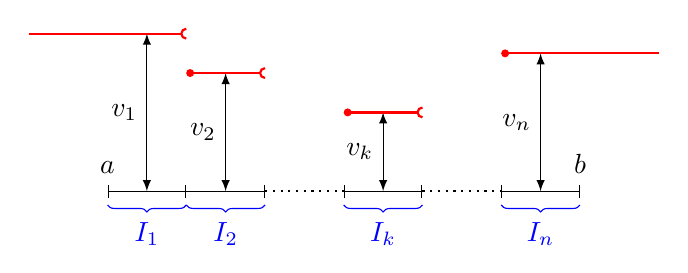
\begin{tikzpicture}
    \draw[int,|-|] (0,0) node[pt]{$a$}-- +(1,0) node[intname]{$I_1$};
    \draw[latex-latex] (0,0) +(.5,0) -- node[left]{$v_1$} +(.5,2) coordinate(v);
    \draw[palier left] (v) +(-1.5,0) -- +(.5,0);

    \draw[int,-|] (1,0) -- +(1,0) node[intname]{$I_2$};
    \draw[latex-latex] (1,0) +(.5,0) -- node[left]{$v_2$} +(.5,1.5) coordinate(v);
    \draw[palier] (v) +(-.5,0) -- +(.5,0);

    \draw[dotted,thick] (2,0) -- +(1,0);

    \draw[int,|-|] (3,0) -- +(1,0) node[intname](Ik){$I_k$};
    \draw[latex-latex] (3,0) +(.5,0) -- node[left]{$v_k$} +(.5,1) coordinate(v);
    \draw[palier] (v) +(-.5,0) -- +(.5,0);

    \draw[dotted,thick] (4,0) -- +(1,0);

    \draw[int,|-|] (5,0) -- +(1,0) node[intname]{$I_n$} node[pt]{$b$};
    \draw[latex-latex] (5,0) +(.5,0) -- node[left]{$v_n$} +(.5,1.75) coordinate(v);
    \draw[palier right] (v) +(-.5,0) -- +(1.5,0);
  \end{tikzpicture}
\end{document}
